\documentclass[a4paper, fontsize=11pt]{scrartcl} % A4 paper and 11pt font 
\usepackage[a4paper,left=3cm,right=2cm,top=2.5cm,bottom=2.5cm]{geometry}

\usepackage[T1]{fontenc} % Use 8-bit encoding that has 256 glyphs
\usepackage{fourier} % Use the Adobe Utopia font for the document - comment this line to return to the LaTeX default
\usepackage[spanish]{babel} % Spanish language/hyphenation
\selectlanguage{spanish}
\usepackage[utf8]{inputenc}
\usepackage{amsmath,amsfonts,amsthm} % Math packages
\usepackage{graphicx} % The graphicx package
\usepackage{placeins}
\usepackage{caption}
\usepackage{subcaption}

\usepackage{hyperref}

\usepackage{cite} % para contraer referencias

\usepackage{listings} % Insert Scripts
\usepackage{color} %red, green, blue, yellow, cyan, magenta, black, white
\definecolor{mygreen}{RGB}{28,172,0} % color values Red, Green, Blue
\definecolor{mylilas}{RGB}{170,55,241}

\lstset{language=Matlab,%
	%basicstyle=\color{red},
	breaklines=true,%
	morekeywords={matlab2tikz},
	keywordstyle=\color{blue},%
	morekeywords=[2]{1}, keywordstyle=[2]{\color{black}},
	identifierstyle=\color{black},%
	stringstyle=\color{mylilas},
	commentstyle=\color{mygreen},%
	showstringspaces=false,%without this there will be a symbol in the places where there is a space
	numbers=left,%
	numberstyle={\tiny \color{black}},% size of the numbers
	numbersep=9pt, % this defines how far the numbers are from the text
	emph=[1]{for,end,break},emphstyle=[1]\color{red}, %some words to emphasise
	%emph=[2]{word1,word2}, emphstyle=[2]{style},    
}

\usepackage{sectsty} % Allows customizing section commands
%\allsectionsfont{\centering \normalfont\scshape} % Make all sections centered, the default font and small caps

\usepackage{fancyhdr} % Custom headers and footers
\pagestyle{fancyplain} % Makes all pages in the document conform to the custom headers and footers
\fancyhead{} % No page header - if you want one, create it in the same way as the footers below
\fancyfoot[L]{} % Empty left footer
\fancyfoot[C]{} % Empty center footer
\fancyfoot[R]{\thepage} % Page numbering for right footer
\renewcommand{\headrulewidth}{0pt} % Remove header underlines
\renewcommand{\footrulewidth}{0pt} % Remove footer underlines
\setlength{\headheight}{13.6pt} % Customize the height of the header

\numberwithin{equation}{section} % Number equations within sections (i.e. 1.1, 1.2, 2.1, 2.2 instead of 1, 2, 3, 4)
\numberwithin{figure}{section} % Number figures within sections (i.e. 1.1, 1.2, 2.1, 2.2 instead of 1, 2, 3, 4)
\numberwithin{table}{section} % Number tables within sections (i.e. 1.1, 1.2, 2.1, 2.2 instead of 1, 2, 3, 4)

%\setlength\parindent{0pt} % Removes all indentation from paragraphs - comment this line for an assignment with lots of text

\newenvironment{myalign}{\par\nobreak\large\noindent\align}{\endalign} %Altering fontsize in equations globally

%----------------------------------------------------------------------------------------
%	TITLE SECTION
%----------------------------------------------------------------------------------------

\newcommand{\horrule}[1]{\rule{\linewidth}{#1}} % Create horizontal rule command with 1 argument of height

\title{	
	\normalfont \normalsize 
	%\textsc{Master en Automática y Robótica - UPM} \\ [25pt] % Your university, school and/or department name(s)
	%\horrule{0.5pt} \\[0.4cm] % Thin top horizontal rule
	\huge Real-Time Cognition \\ % The assignment title
	%\horrule{2pt} \\[0.5cm] % Thick bottom horizontal rule
}

\author{Jorge Camarero Vera - 07052} % Your name

\date{\normalsize\today} % Today's date or a custom date

\begin{document}
	\maketitle
	
	La computación en \textbf{tiempo real} describe sistemas de hardware y sofware sujetos a restricciones de tiempo real. Los sistemas de tiempo real deben garantizar una respuesta dentro de unas restricciones específicas de tiempos, a menudo referidas como "deadline". Las respuestas de tiempo real son a menudo entendidas para actuar en el orden de los milisegundos, y a veces en microsegundos\footnote{Esta información está sacada del primer párrafo de la entrada de wikipedia de \href{https://en.wikipedia.org/wiki/Real-time_computing}{Real-time computing}}.\\
	
	Con esta descripción dada vemos que las respuestas en tiempo deben ser dadas dentro de un tiempo estipulado. Un robot en el que se ha implementado una arquitectura cognitiva de tiempo real debe actuar en tiempos de la acción humana, la escala de los tiempos de la acción humana vienen detallados en la Figura \ref{Times} . Sabiendo que los sistemas de tiempo real actual en el orden de los milisegundos o por debajo se puede dividir la Figura \ref{Times} en dos partes, por encima de acciones deliberadas y por debajo, éstas últimas serían respuestas con restricciones de tiempo real.\\
	
	\begin{figure}[h!]
		\centering
		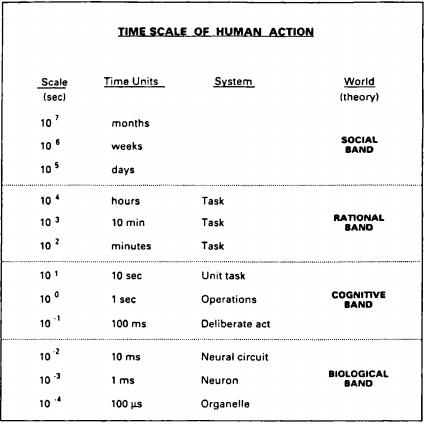
\includegraphics[width=0.5\linewidth]{images/Time.png}
		\caption{Escala de tiempo de la acción humana, descrita por Newell\cite{TIMES}.}
		\label{Times}
	\end{figure}
	\FloatBarrier
	
	La arquitectura cognitiva \textbf{LIDA}\cite{LIDA} permite atención, selección de la acción y aprendizaje como un humano destinado a ser utilizado en el control de agentes cognitivos que replican experimentos humanos, así como la realización de tareas del mundo real. Implementa principalmente \textit{Global Workspace Theory}\cite{GWT}. LIDA está basado en el ciclo cognitivo de LIDA\ref{LIDA}, un ciclo puede ser interpretado como un momento de la cognición. Procesos cognitivos de alto nivel están compuestos por muchos de estos ciclos cognitivos.\\
	
	\begin{figure}[h!]
		\centering
		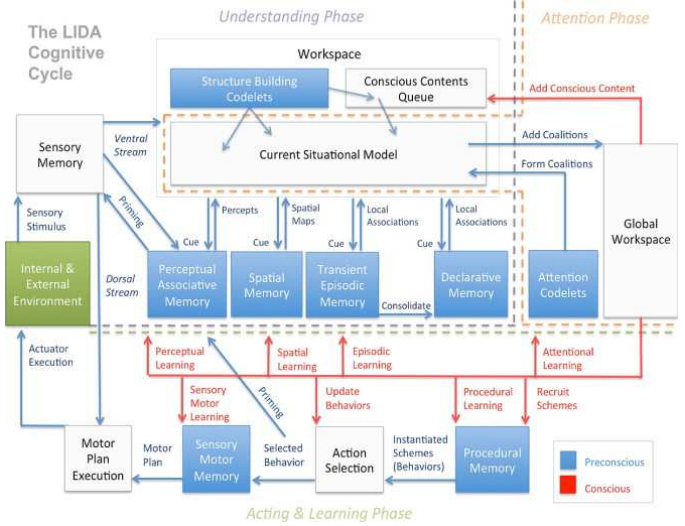
\includegraphics[width=0.8\linewidth]{images/LIDA.png}
		\caption{Diagrama del ciclo cognitivo de LIDA\cite{LIDA}.}
		\label{LIDA}
	\end{figure}
	\FloatBarrier
	
	Cada ciclo cognitivo tarda entorno a \textbf{$300\,ms$}. Por tanto, en LIDA los modos de selección de la acción operan a diferentes escalas de tiempos:
	
	\begin{itemize}
		\item  Acciones meditadas conscientemente son seleccionadas entre cinco o diez veces por segundo (\textbf{$100-200\,ms$}).
		\item La voluntad puede tomar segundos, o incluso mucho más.
		\item Acciones automatizadas son tan rápidas como un ciclo cognitivo (\textbf{$300\,ms$}) o incluso más rápidas.
		\item  Los mecanismos de alarma operan por debajo de los \textbf{$50\,ms$}.
		\item La ejecución de una acción requiere comunicación sensitiva-motora y ocurre de diez a cuarenta veces por segundo (\textbf{$25-100\,ms$})
	\end{itemize}
	
	Con estos datos se ve que el funcionamiento de acciones en LIDA ocurren por debajo de los segundos, algunas bajando hasta las decenas de milisegundos. Por tanto \textbf{los robots que implementarían LIDA podrían actuar en tiempo real}. El problema puede venir que $300\,ms$ para un ciclo cognitivo puede ser alto para mantener comportamientos en tiempo real cuando se implementan procesos cognitivos de alto nivel que requieran varios ciclos cognitivos.\\
	
	LIDA es principalmente empleado como agente de información humana, pero también puede funcionar en un robot físico, su reactividad facilitada por operaciones asíncronas y aprendizaje \textit{one-shot} en \textit{Sparse Distributed Memory, SDM}. Aún así, LIDA ha sido poco validada en causalidad y probabilidad, ambos son importantes para aplicaciones del mundo real como la robótica.\\
	
	Como casos distintos a LIDA se tienen las arquitecturas \textbf{4D-RCS}\cite{4DRCS} y \textbf{Subsumption}\cite{SUBSUMPTION}, ambas han sido implementadas en robots autónomos, en mayor medida \textit{4D-RCS}. Como su nombre indica \textit{Real-time Control System, RCS} es una arquitectura cognitiva de tiempo real diseñada para cualquier nivel de comportamiento inteligente, incluso a niveles de desempeño humano.\\
	
	Como se puede ver en la Figura \ref{RCS}, en RCS las tres capas inferiores se pueden considerar como sistemas de tiempo real, sobretodo los planificadores de servos que actúan en torno a $50\,ms$.\\
	
	\begin{figure}[h!]
		\centering
		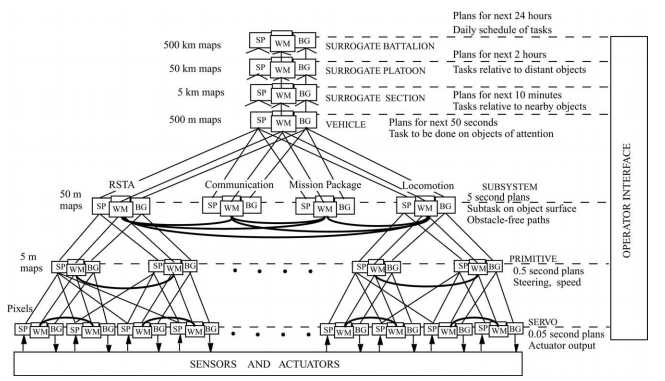
\includegraphics[width=0.8\linewidth]{images/RCS.png}
		\caption{Modelo de referencia de la arquitectura 4D/RCS para vehículos militares autónomos\cite{4DRCS}.}
		\label{RCS}
	\end{figure}
	\FloatBarrier
	
	Debido a sus capacidades de tiempo real, RCS permite construir vehículos autónomos como \textit{Demo III experimental unmanned ground vehicle (XUV)}, se han llevado a cabo tests en terrenos no estructurados, bosques, con hierva alta, lagos, etc, y recorrido distancias desde los $500\,m$ hasta los $2.000\,m$. Por tanto, mediante RCS se pueden diseñar robots que trabajen en el mundo real a nivel prácticamente humano.\\
	
	En cuanto a \textbf{SOAR}\cite{SOAR} es una arquitectura basada en la hipótesis de que todos los comportamientos orientados a un fin deliberados pueden ser llamados como la selección y aplicación de operadores a un estado, dicho estado es una representación de la actual situación a resolver. SOAR tiene memorias separadas para descripciones de su actual situación y de su conocimiento a largo plazo.\\
	
	Cuando SOAR interacciona con el entorno\cite{ARCHITECTURES}, debe hacer uso de una mecanismo que le permita efectuar cambios en el entorno; el mecanismo empleado por SOAR es llamado \textit{output functions}. En el caso de una salida de comando de motor en SOAR, la cuál no puede ser directamente ejecutada en el mundo real, un programa externo es siempre necesario para manejar la ejecución real por SOAR. Por tanto, SOAR es incapaz por sí mismo de tares en Tiempo Real con un entorno del \textit{mundo real}. Aún así se ha implementado en robots autónomos\cite{SOARROBOT}. 
	
	\bibliographystyle{acm} % estilo de la bibliografía.
	\bibliography{yyyy} 
	
	\begin{thebibliography}{X}
		
		\bibitem{TIMES} \textsc{A. Newell}, \textit{Unified Theories of Cognition (The William James Lectures)}, Harvard University Press, Cambridge, MA, 1990.
		
		\bibitem{LIDA} \textsc{S. Franklin, T. Madl, S. D'mello} y \textsc{J. Snaider}, \textit{LIDA: A Systems-level Architecture for Cognition, Emotion, and Learning}, Autonomous Mental Development, IEEE Transactions on  (Volume:6 ,  Issue: 1 ), 2014.
		
		\bibitem{GWT} \textsc{Bernard J. Baars} y \textsc{Stan Franklin}, \textit{Consciousness is Computational: The LIDA Model of Global Workspace Theroy}, International Journal of Machine Consciousness.
		
		\bibitem{4DRCS} \textsc{James S. Albus} y \textsc{Anthony J. Barbera}, \textit{RCS: A Cognitive Architecture for Intelligent Multi-Agent Systems}, Annual Reviews in COntrol, 2005.
		
		\bibitem{SUBSUMPTION} \textsc{Rodney A. Brooks}, \textit{A Robust Layered Control System for a Mobile Robot}, IEEE Journal of Robotics and Automation, VOL. RA-2, 1986.
		
		\bibitem{SOAR} \textsc{Jill F. Lehman, John Laird} y \textsc{Paul Rosenbloom}, \textit{A Gentle Introduction to SOAR, an Architecture for Human Cognition: 2006 Update}, 2006.
		
		\bibitem{ARCHITECTURES} \textsc{Daqi Dong} y \textsc{Stan Franklin}, \textit{The Action Execution Process Implemented in Diferent Cognitive Architectures: A Review}, Journal of Artificial General Intelligence, 2014.
		
		\bibitem{SOARROBOT} \textsc{Scott D. Hanford, Oranuj Janrathistikarn} y \textsc{Lyle N. Long}, \textit{Control of Mobile Robots Using the SOAR Cognitive Architecture}, Journal of aerospace computing, information, and communication, Vol 6, Febrero 2009.
		
	\end{thebibliography}
	
 	
\end{document}